\documentclass{article}
% Choose a conveniently small page size
% PACKAGES
\usepackage[margin = 1in]{geometry}
\usepackage{amsfonts}
\usepackage{amsmath}
\usepackage{amssymb}
\usepackage{multicol}
\usepackage{graphicx}
\usepackage{float}
\usepackage{xcolor}
\usepackage{amsthm}
\usepackage{dsfont}
\usepackage{hyperref}
\usepackage{subcaption}
\usepackage{listings}

\lstset{
  language=Python,
  basicstyle=\ttfamily\small,
  keywordstyle=\color{blue},
  stringstyle=\color{red},
  commentstyle=\color{olive},
  morecomment=[l][\color{magenta}]{\#},
  showstringspaces=false
}

% MACROS
% Set Theory
\def\N{\mathbb{N}}
\def\R{\mathbb{R}}
\def\C{\mathbb{C}}
\def\Z{\mathbb{Z}}
%\def\^{\hat}
\def\-{\vec}
\def\d{\partial}
\def\!{\boldsymbol}
\def\X{\times}
%\def\-{\bar}
\def\bf{\textbf}
\def\l{\left}
\def\r{\right}
\title{Weekly Report}
\author{Damien Beecroft}
\begin{document}
\maketitle
% \newpage
\section{Introduction}
The code for the time stepping scheme presented last week diverges in the same way as the Lax-Friedrichs fast sweeping (LFFS) method. So, it appears that the problem is how I am handling the collision operator. In this report we play with the collision operator a bit to see whether we can determine what is going awry.
\section{Progress}
\subsection{Implicit Discretization Methods}
In previous reports we analyzed the convergence behavior of the Lax-Friedrichs fast sweeping method
\[
    v \frac{f_i^{(l+1)} - f_{i-1}^{(l+1)}}{\Delta x} = Q^+(f^{(l)}, f^{(l)}) - C \rho_i^{(l)} f_i^{(l+1)}
\]
and the time stepping method
\begin{gather*}
    \frac{f_i^* - f_i^{(l)}}{\Delta t} + v \frac{f_i^{(l)} - f_{i-1}^{(l)}}{\Delta x} = 0\\
    \frac{f_i^{(l+1)} - f^*_i}{\Delta t} = Q^+(f^*,f^*) - C \rho_i^* f^*_i.
\end{gather*}
Both of these methods diverged with a large hump forming on the left of the solution. It appears that there is an issue with how I am handling the collision operator.
\subsection{Explicit Discretization Methods}
I changed how we handle the collision operator in the code. This change should give an equivalent steady state solution. The altered LFFS method is
\[
    v \frac{f_i^{(l+1)} - f_{i-1}^{(l+1)}}{\Delta x} = Q(f^{(l)}, f^{(l)}).
\]
This produces the update scheme 
\[
    f_i^{(l+1)}  = \frac{\Delta x}{v} Q(f^{(l)}, f^{(l)}) + f_{i-1}^{(l+1)}.
\]
This method gives the following results.
\begin{figure}[H]
    \centering
    \begin{subfigure}[b]{0.45\textwidth}
    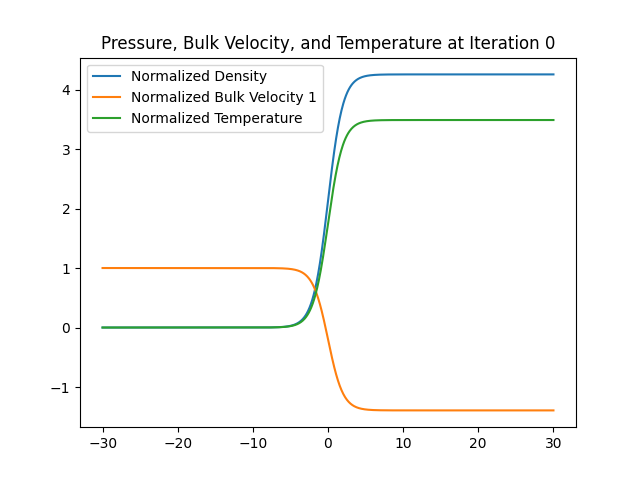
\includegraphics[width=\textwidth]{imgs/lax_friedrichs/iter0.png}
        % \caption{Image 1}
        % \label{fig:image1}
    \end{subfigure}
    \hfill
    \begin{subfigure}[b]{0.45\textwidth}
    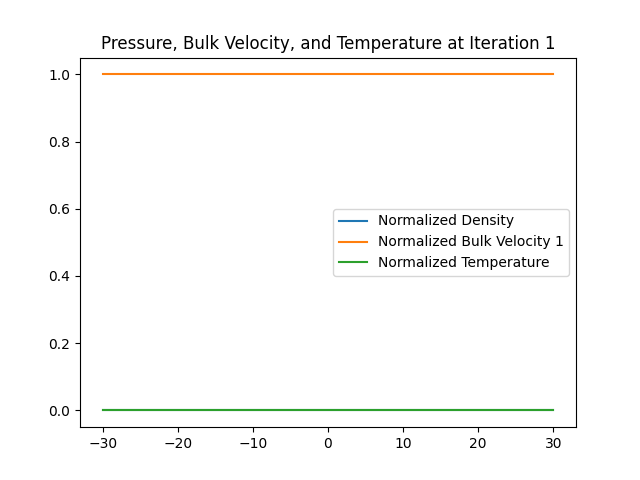
\includegraphics[width=\textwidth]{imgs/lax_friedrichs/iter1.png}
        % \caption{Image 2}
        % \label{fig:image2}
    \end{subfigure}
    
    \vspace{1em} % Add some vertical space between the rows
    
    \begin{subfigure}[b]{0.45\textwidth}
    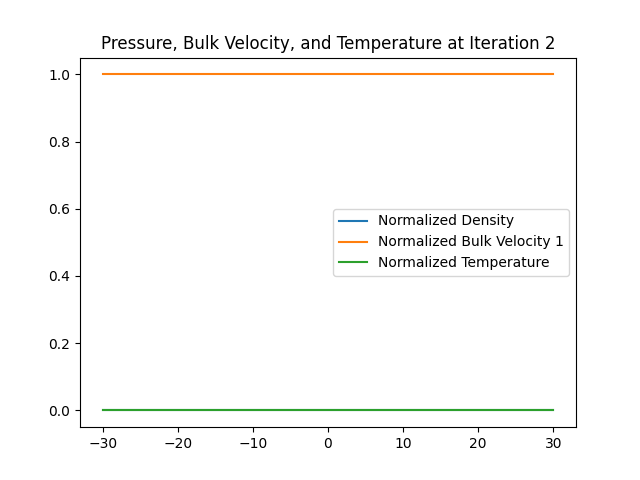
\includegraphics[width=\textwidth]{imgs/lax_friedrichs/iter2.png}
        % \caption{Image 3}
        % \label{fig:image3}
    \end{subfigure}
    % \hfill
    % \begin{subfigure}[b]{0.45\textwidth}
    % \includegraphics[width=\textwidth]{imgs/lax_friedrichs/iter150.png}
    %     % \caption{Image 4}
    %     \label{fig:image4}
    % \end{subfigure}
    
    \caption{Above are the normalized values of the density, bulk velocity, and temperature for iterations zero, one, and two from the LFFS method. The values are plotted synonymously to how they are plotted in Figure 2 of \textit{An adaptive dynamical low rank method for the nonlinear Boltzmann equation} by Hu et al. The solution settles to a flat line immediately.}
    % \label{fig:four_images}
\end{figure}
The values of $Q(f^{(l)}, f^{(l)})$ are very small in comparison to the values of $f^{(l)}$, so the update scheme is essentially
\[
    f_i^{(l+1)} = f_{i-1}^{(l+1)}.
\]
This is why we are getting an almost constant solution.
The altered time-stepping discretization is 
\begin{gather*}
    \frac{f_i^* - f_i^{(l)}}{\Delta t} + v \frac{f_i^{(l)} - f_{i-1}^{(l)}}{\Delta x} = 0\\
    \frac{f_i^{(l+1)} - f^*_i}{\Delta t} = Q(f^*,f^*).
\end{gather*}
This produces the update scheme
\begin{gather*}
    f_i^* = \left(1 - \frac{v \Delta t}{\Delta x} \right)f_i^{(l)} + \frac{v \Delta t}{\Delta x}  f_{i-1}^{(l)}\\
    f_i^{(l+1)} = f^*_i + \Delta t Q(f^*,f^*).
\end{gather*}
Using the time-stepping scheme the solution settles to exactly the same form.
\begin{figure}[H]
    \centering
    \begin{subfigure}[b]{0.45\textwidth}
    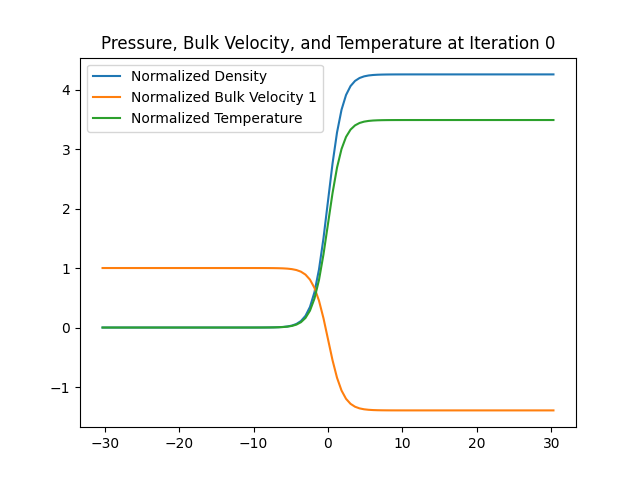
\includegraphics[width=\textwidth]{imgs/time_stepping/iter0.png}
        % \caption{Image 1}
        \label{fig:image1}
    \end{subfigure}
    \hfill
    \begin{subfigure}[b]{0.45\textwidth}
    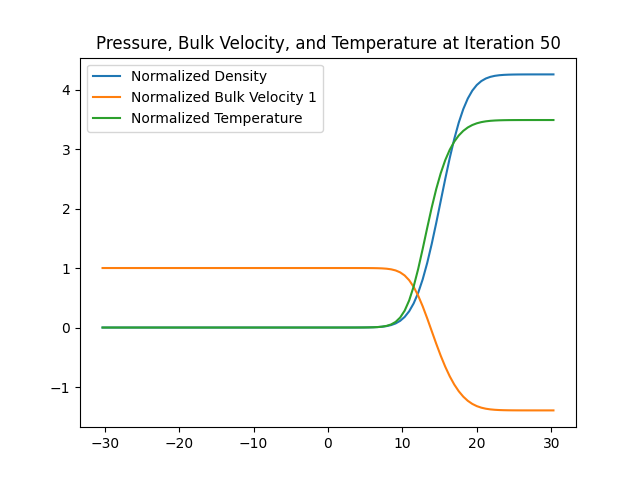
\includegraphics[width=\textwidth]{imgs/time_stepping/iter50.png}
        % \caption{Image 2}
        \label{fig:image2}
    \end{subfigure}
    
    \vspace{1em} % Add some vertical space between the rows
    
    \begin{subfigure}[b]{0.45\textwidth}
    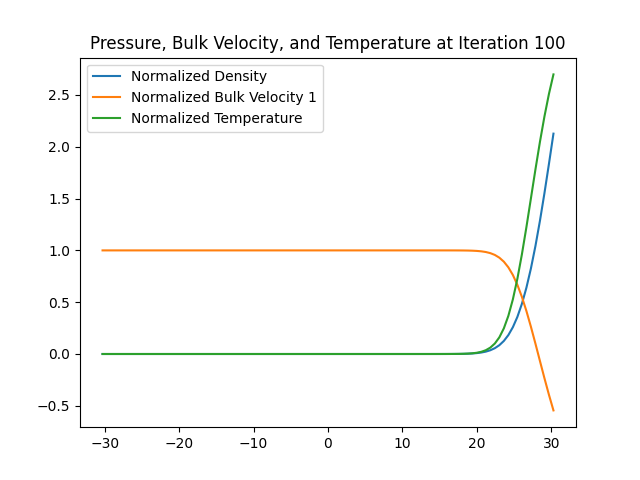
\includegraphics[width=\textwidth]{imgs/time_stepping/iter100.png}
        % \caption{Image 3}
        \label{fig:image3}
    \end{subfigure}
    \hfill
    \begin{subfigure}[b]{0.45\textwidth}
    \includegraphics[width=\textwidth]{imgs/time_stepping/iter150.png}
        % \caption{Image 4}
        \label{fig:image4}
    \end{subfigure}
    
    \caption{Above are the normalized values of the density, bulk velocity, and temperature for iterations zero, one, and two from the LFFS method. The values are plotted synonymously to how they are plotted in Figure 2 of \textit{An adaptive dynamical low rank method for the nonlinear Boltzmann equation} by Hu et al. The solution advects to the right until the solution on the interior is constant, just as we saw in the LFFS method.}
    \label{fig:four_images}
\end{figure}
Again, this behavior is due to the fact that the values of $Q(f^{(l)}, f^{(l)})$ are very small in comparison to the values of $f^{(l)}$.
\section{To Do For Next Week}
It is apparent from this report that the explicit and implicit discretizations are not modeling the same physical scenario. Furthermore, neither of them are converging to the solution illustrated in Figure 2 of \textit{An adaptive dynamical low rank method for the nonlinear Boltzmann equation} by Hu et al. I need to go through the \verb|CBoltz2_Carl_Maxwell| code to understand how it can be correctly applied to the problem at hand. It is obvious that I am using it incorrectly somehow.
\end{document}

% We first try changing how we implement the collision operator in the equation to see if this affects the divergence of the solution. The discretization that we dealt with before was
% \begin{gather*}
%     \frac{f_i^* - f_i^{(l)}}{\Delta t} + v \frac{f_i^{(l)} - f_{i-1}^{(l)}}{\Delta x} = 0\\
%     \frac{f_i^{(l+1)} - f^*_i}{\Delta t} = Q^+(f^*,f^*) - C \rho_i^* f^*_i.
% \end{gather*}
% For this implementation I had to change Jingwei's \verb|CBoltz2_Carl_Maxwell| method to only return the gain term in the collision operator. I called this new function \verb|Qplus|. The new discretization would simply be
% \begin{gather*}
%     \frac{f_i^* - f_i^{(l)}}{\Delta t} + v \frac{f_i^{(l)} - f_{i-1}^{(l)}}{\Delta x} = 0\\
%     \frac{f_i^{(l+1)} - f^*_i}{\Delta t} = Q(f^*,f^*).
% \end{gather*}
% This simplifies to 
% \begin{gather*}
%     f_i^* = \left(1 - \frac{v \Delta t}{\Delta x} \right)f_i^{(l)} + \frac{v \Delta t}{\Delta x}  f_{i-1}^{(l)}\\
%     f_i^{(l+1)} = f^*_i + \Delta t Q(f^*,f^*).
% \end{gather*}
% For the LFFS method, the original method that we tried was 
% \[
%     v \frac{f_i^{(l+1)} - f_{i-1}^{(l+1)}}{\Delta x} = Q^+(f^{(l)}, f^{(l)}) - C \rho_i^{(l)} f_i^{(l+1)}.
% \]
% Now, we deal with a different discretization:
% \[
%     v \frac{f_i^{(l+1)} - f_{i-1}^{(l+1)}}{\Delta x} = Q(f^{(l)}, f^{(l)}).
% \]
% This produces the scheme
% \[
%     f_i^{(l+1)}  = \frac{\Delta x}{v} Q(f^{(l)}, f^{(l)}) + f_{i-1}^{(l+1)}.
% \]